\documentclass[10pt]{article}

\usepackage{float}
\usepackage[T1]{fontenc}
\usepackage[utf8]{inputenc}
\usepackage[english]{babel}
\usepackage{amssymb,amsfonts,amsmath,amsthm}
\usepackage{graphicx}
\usepackage{lmodern}
\usepackage{mdframed}
\usepackage{hyperref}
\usepackage{cases}
\usepackage{framed}
\usepackage{pdfpages}
\usepackage{multicol}
\usepackage[margin=60pt]{geometry}
\usepackage{abstract}
\renewcommand{\abstractnamefont}{\normalfont\Large\bfseries}
\renewcommand{\abstracttextfont}{\normalfont\normalsize}

\usepackage{pgfplots}
%\usepgfplotslibrary{colormaps}
\pgfplotsset{every axis/.append style={line width=1pt}}

\usepackage{adjustbox}
\newcommand{\specialcell}[2][c]{%
	\begin{tabular}[#1]{@{}c@{}}#2\end{tabular}}

\newcommand{\avg}[1]{\left< #1 \right>} % for average
\newcommand{\Ne}{N_\mathrm{e}}

% \renewcommand{\baselinestretch}{2}

\begin{document}
\includepdf[pages={1}]{frontpage.pdf}
	\begin{abstract}
		Adaptation in protein-coding sequences can be detected using multiple sequence alignments across species (inter-specific data). This method uses phylogenetic codon models, classically formulated in terms of the relative synonymous and non-synonymous substitution rates. However, because of the background of purifying selection, these models are limited in their sensitivity. Recent developments, have led to more sophisticated mutation-selection codon models aiming at making a more detailed quantitative assessment of the interplay between mutation, purifying and positive selection, leading to potentially more powerful and more quantitative detection of adaptation.
		In this study, I first conducted an analysis on placental mammals protein-coding sequences, and assessed the performance of mutation-selection codon models to detect protein under adaptation. Out of the $1,355$ sequences of the dataset, the method detected $27$ proteins under adaptation. These proteins were enriched in ontology terms related to immune processes.
		Adaptation in protein-coding sequences can also be detected by combining divergence and polymorphism (intra-specific) data. Thus, I developed a pipeline to integrate inter- and intra-specific data across the entire exome. This pipeline was applied to a dataset of \textit{Homo sapiens} polymorphism, and showed that the set of proteins detected to be under adaptation globally over mammals showed marginally significant increase in the rate of adaption inferred using \textit{Homo sapiens} polymorphism. This relatively weak correlation might just reflect reflect the limited statistical power of the analysis. However, it is also possible that the two methods are inherently testing for different patterns of adaptation.  \\
		
		\noindent \textbf{Keywords.} Evolution, Adaptation, Coding Sequences, Codon models, Synonymous/Non-synonymous substitutions.
	\end{abstract}
	\vspace*{20pt}
	\begin{multicols}{2}
	\section*{Introduction}

	Molecular sequences are shaped over time by different evolutionary forces such as mutation, selection and random drift \cite{ohta_nearly_1992}. Selection takes a variety of forms since a mutation in a molecular sequence can either be neutral, positively or negatively selected. More globally, different proteins might be in different selection regimes. Some, mostly under strong purifying selection, are expected to be stable trough time.
	Other proteins, involved in a arm race as for example against pathogens, are under recurrent positive selection and tend to evolve faster \cite{enard_viruses_2016}. One main goal of molecular evolution is to quantify the intensity of evolutionary forces acting on sequences, and to detect the signature in present-day sequences left by recurrent events of positive selection. \\
	
	Theoretically, in order to detect positive selection, one must have data where part of the sequence is known to be under a neutral regime, which can be used as a null model. In the case of protein-coding DNA sequences, a mutation will either be synonymous (not changing the translated amino-acid), or non-synonymous (such that the translated amino-acid will be different). Synonymous sites are usually taken as proxies for neutral sites, although they may be under weak selection. Non-synonymous mutations, on the other hand, are under a mixture of adaptation, purifying selection and random drift, depending on the selection coefficient associated with the new amino-acid. The synonymous sites are used to quantify the neutral process, and the deviation to this neutral process on non-synonymous sites gives insight on the strength of both positive and purifying selection. \\
	
	Contrasting synonymous and non-synonymous changes, two different types of methods have emerged to quantify both positive and purifying selection acting on protein-coding sequences.
	One method, stemming from population genetics, contrasts polymorphism inside a population (intra-specific data) and divergence to a close species. In the following, this method will be called population-based method. Another method, stemming from phylogeny, uses multiple sequence alignment (inter-specific data) in different species to quantify adaptation. This method will be called phylogeny-based method. One goal of the present work is to confront these two types of approaches.\\
	
	\begin{figure*}[hb!]
		\begin{mdframed}
			\centering
			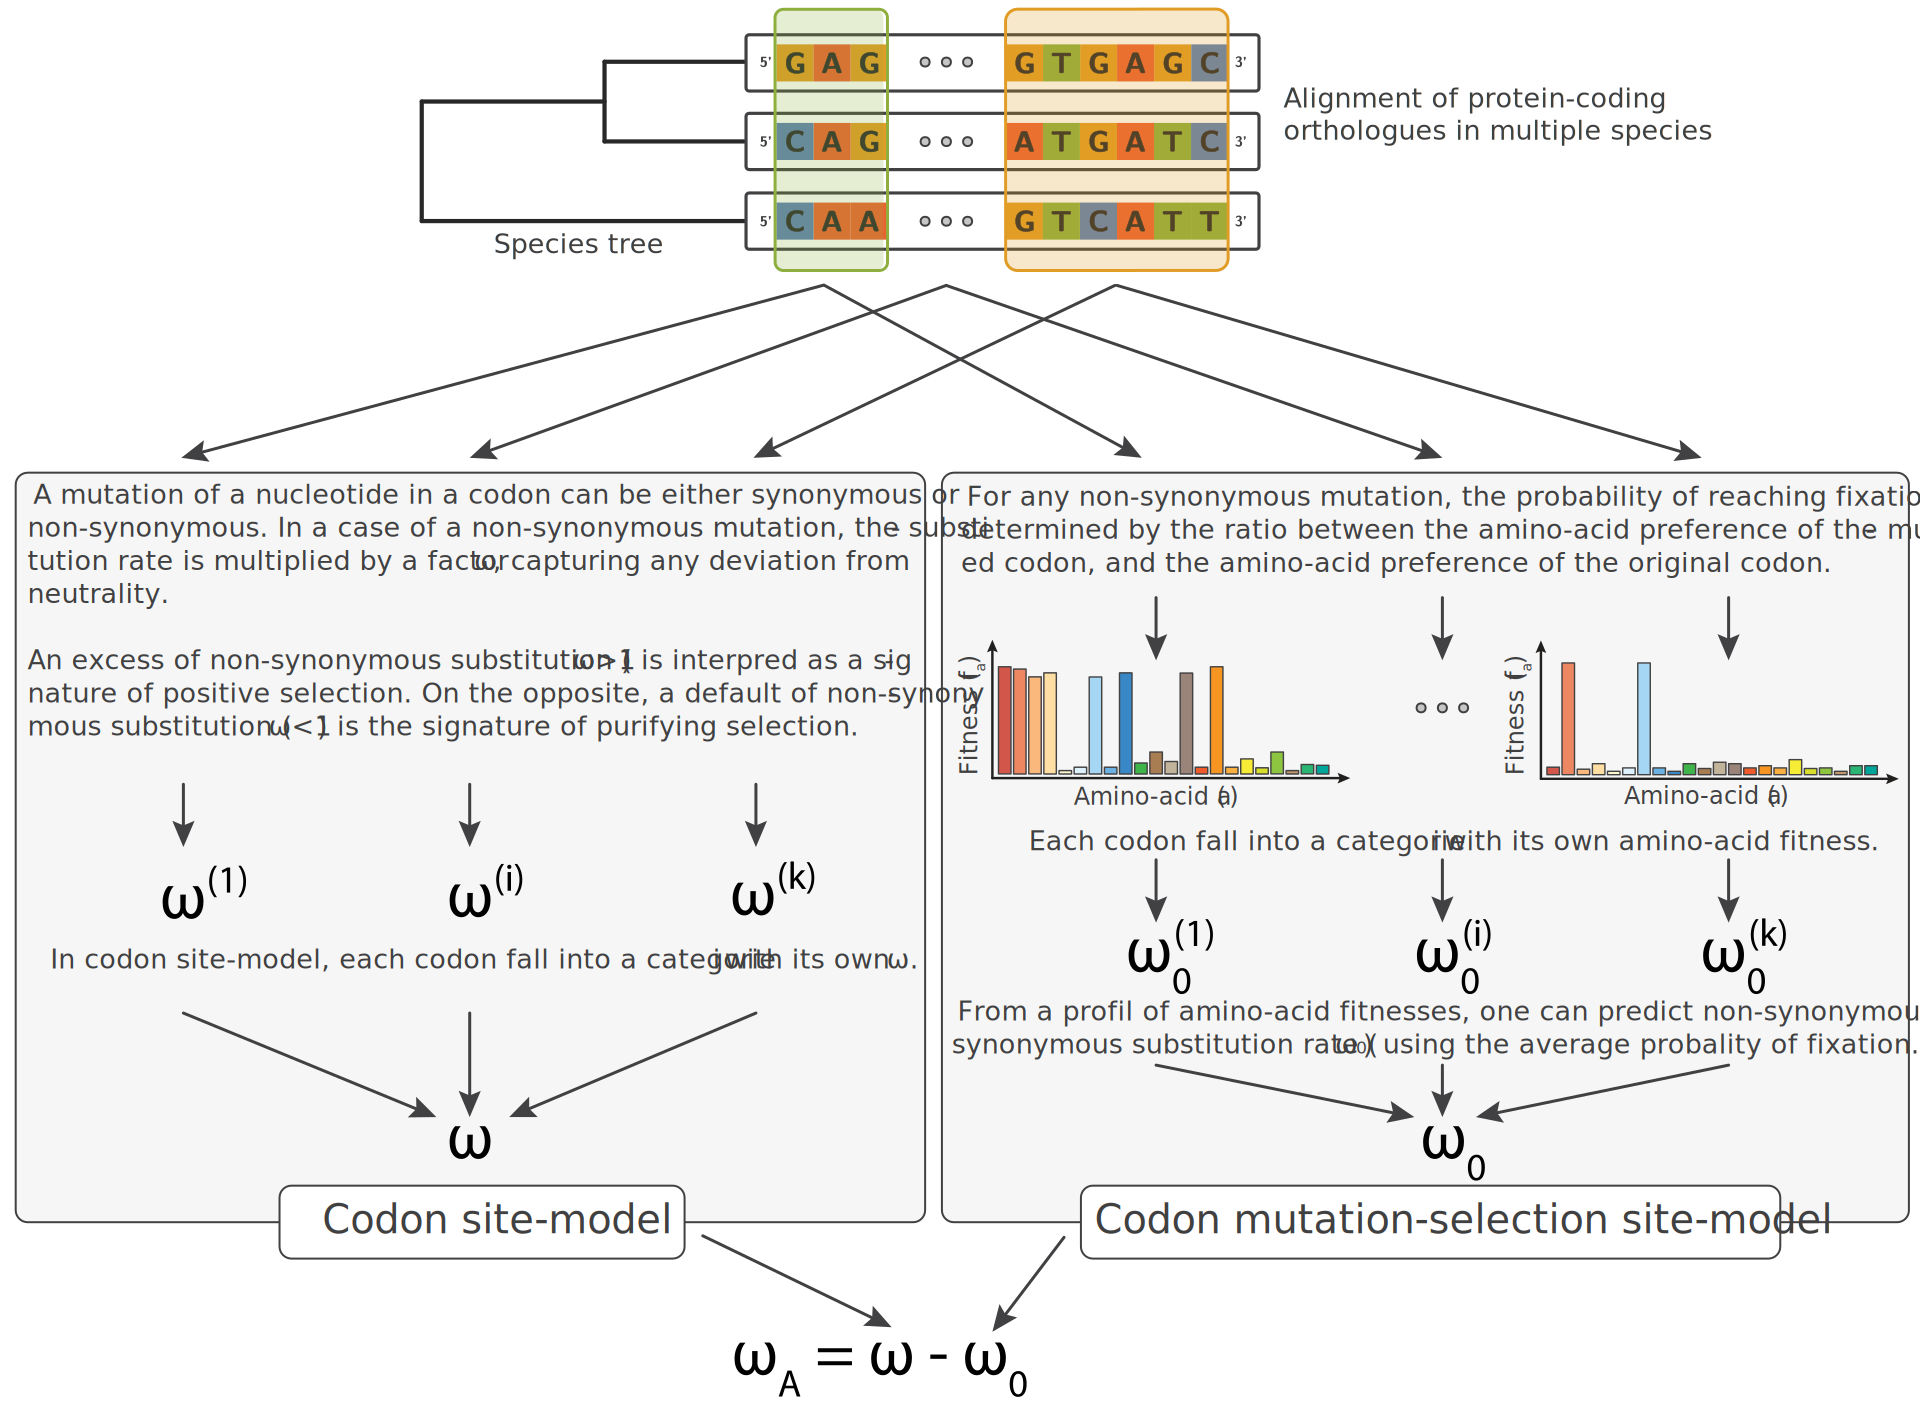
\includegraphics[width=\textwidth]{../Figures/codon_model.pdf}\\
			\caption{ \textbf{$\omega_A$ estimation with mutation-selection codon model}. On the left panel, the codon site-model estimates $\omega$, the rate of non-synonymous over synonymous substitutions, as the average of $\omega^{(i)}$ at each site. On the right panel, the mutation-selection codon model estimates the fitness of each amino-acid at each site. From the set of site-specific amino-acid fitness profiles, one can compute $\omega_{0}$ which is the predicted rate of non-synonymous over synonymous substitution at the mutation-selection balance and genuinely taking into account purifying selection. Both methods runs independently from the same alignment data. From these two independent runs, $\omega_A$ is computed as the difference $\omega - \omega_{0}$\label{fig:codon_model}}
		\end{mdframed}
	\end{figure*}

	In population-based method, one of the most widely used test for adaptation was proposed by McDonald and Kreitman \cite{McDonald1991}. This method uses the substitutions (mutations that reach fixation) between two close species and polymorphism (sites with at least two alleles) inside on population. Under a neutral regime, deleterious mutations are assumed to occur, but are quickly removed by selection, and the ratio of non-synonymous substitutions over synonymous substitutions ($d_N/d_S$) is expected to be lower than one, since none of non-synonymous deleterious mutations will reach fixation. Also the ratio of non-synonymous polymorphism over synonymous polymorphism ($p_N/p_S$) is also expected to be lower than one, since the non-synonymous deleterious mutations will be removed quickly from the population. Most importantly, in the absence of advantageous mutations, these two ratio are expected to be the same ($d_N/d_S=p_N/p_S$). If advantageous mutations occur, then they are fixed rapidly in the population, thus contributing solely to divergence but not to polymorphism, leading to an overall $d_N/d_S$ greater than $p_N/p_S$ \cite{smith_adaptive_2002, kimura_neutral_1983}. In the end, the method can therefore leads to a decomposition in the total rate rate of evolution ($d_N/d_S$) into two components: respectively neutral ($p_N/p_S$) and adaptive ($d_N/d_S-p_N/p_S$). This method is however plagued by the presence of moderately deleterious non-synonymous mutations, which can segregate at substantial frequency in the population without reaching fixation, thus contributing solely to polymorphism, and not to divergence, potentially resulting on an under-estimation of the rate of adaptive evolution \cite{eyre-walker_quantifying_2002}. Subsequent developments have tried to correct for this effect be relying on an explicit \textit{nearly-neutral model}, so as to derive the expected value of $d_N/d_S$ and $p_N/p_S$ in the absence of adaptation. The observed deviation of $d_N/d_S$ compared to this null expectation then provides an estimate of the rate of adaptation \cite{eyre-walker_estimating_2009, galtier_adaptive_2016}. \\

	The phylogeny-based method models the substitution rate at the codon level. Synonymous and non-synonymous mutations are treated differently. The rate of non-synonymous substitutions over the rate of synonymous substitutions (denoted $\omega=d_N/d_S$) is estimated as a parameter of the model \cite{Muse1994,Goldman1994}. Assuming synonymous mutations are neutral, an $\omega>1$ signals an excess in the rate of non-synonymous substitutions, indicating that the protein is under adaptive evolution. Conversely, a default of non-synonymous substitutions, leading to $\omega<1$, means the protein is under purifying selection. However, in practice, protein are typically under a mix of adaptation and purifying selection, thus typically leading to an $\omega<1$ even in the presence of positive selection. More sophisticated methods have been proposed. In particular, site-models trying to detect specific site of the sequence with an $\omega>1$, have been developed \cite{Yang2001, kosiol_patterns_2008}.
	However these models potentially miss a substantial fraction of adaptation and do not quantify the rate of adaptation.  \\
	
	An alternative approach to codon site-models would be to do as in the case of population-based method mentioned above, to rely on an explicit \textit{nearly-neutral model} as the null model against which to detect deviation of $\omega=d_N/d_S$. A recent development in this direction, the so-called phylogenetic mutation-selection models, provide a null model by estimating the fitness landscape over amino-acid sequences \cite{Yang2008, Halpern1998, Rodrigue2010}. At the mutation-selection balance, the codons will bounce between amino-acids with high fitnesses, and mutation from a high fitness amino-acid towards a low fitness amino-acid will have a small probability of fixation. Thus the model genuinely takes into account purifying selection. By contrasting $\omega$ estimated by the classical codon models and the $\omega$ predicted by the mutation-selection model, one can hope to extract the rate of adaption, but this has not yet been conducted on a large scale \cite{Rodrigue2016}. \\
	
	The population- and phylogeny-based method work over very different time scales.
	For that reason, they might be capturing different signals: isolated events of adaptation along a particular lineage for population-based method, versus long-term evolutionary Red-Queen for phylogeny based methods. On the other hand, the two signals might be correlated. This represent a unique opportunity to confound these two types of approaches on non-overlapping data frames. Accordingly, the goal of this study is to set-up a pipeline for gathering divergence and polymorphism data for coding genes across species. As a proof of concept, I analyzed 1,355 protein-coding sequences (CDS) orthologs in mammals, and conducted two separate analysis on these CDS. First, alignments in placentals (except \textit{Homo sapiens} and \textit{Pan troglodytes}) were used to run classical site-models and mutation-selection models. The method estimated the rate of adaptation in each CDS, and extracted CDS with a rate of adaptation significantly high. Secondly, the population-based method was conducted using polymorphism available in \textit{Homo sapiens} and divergence to \textit{Pan troglodytes}. The pipeline then testes if the group of sequences detected with a high rate of adaption in the phylogeny-based method also display a high rate of adaptation in the population-based method.

	\section*{Materials and methods}


	\begin{figure*}[hb!]
	\begin{mdframed}
		\centering
		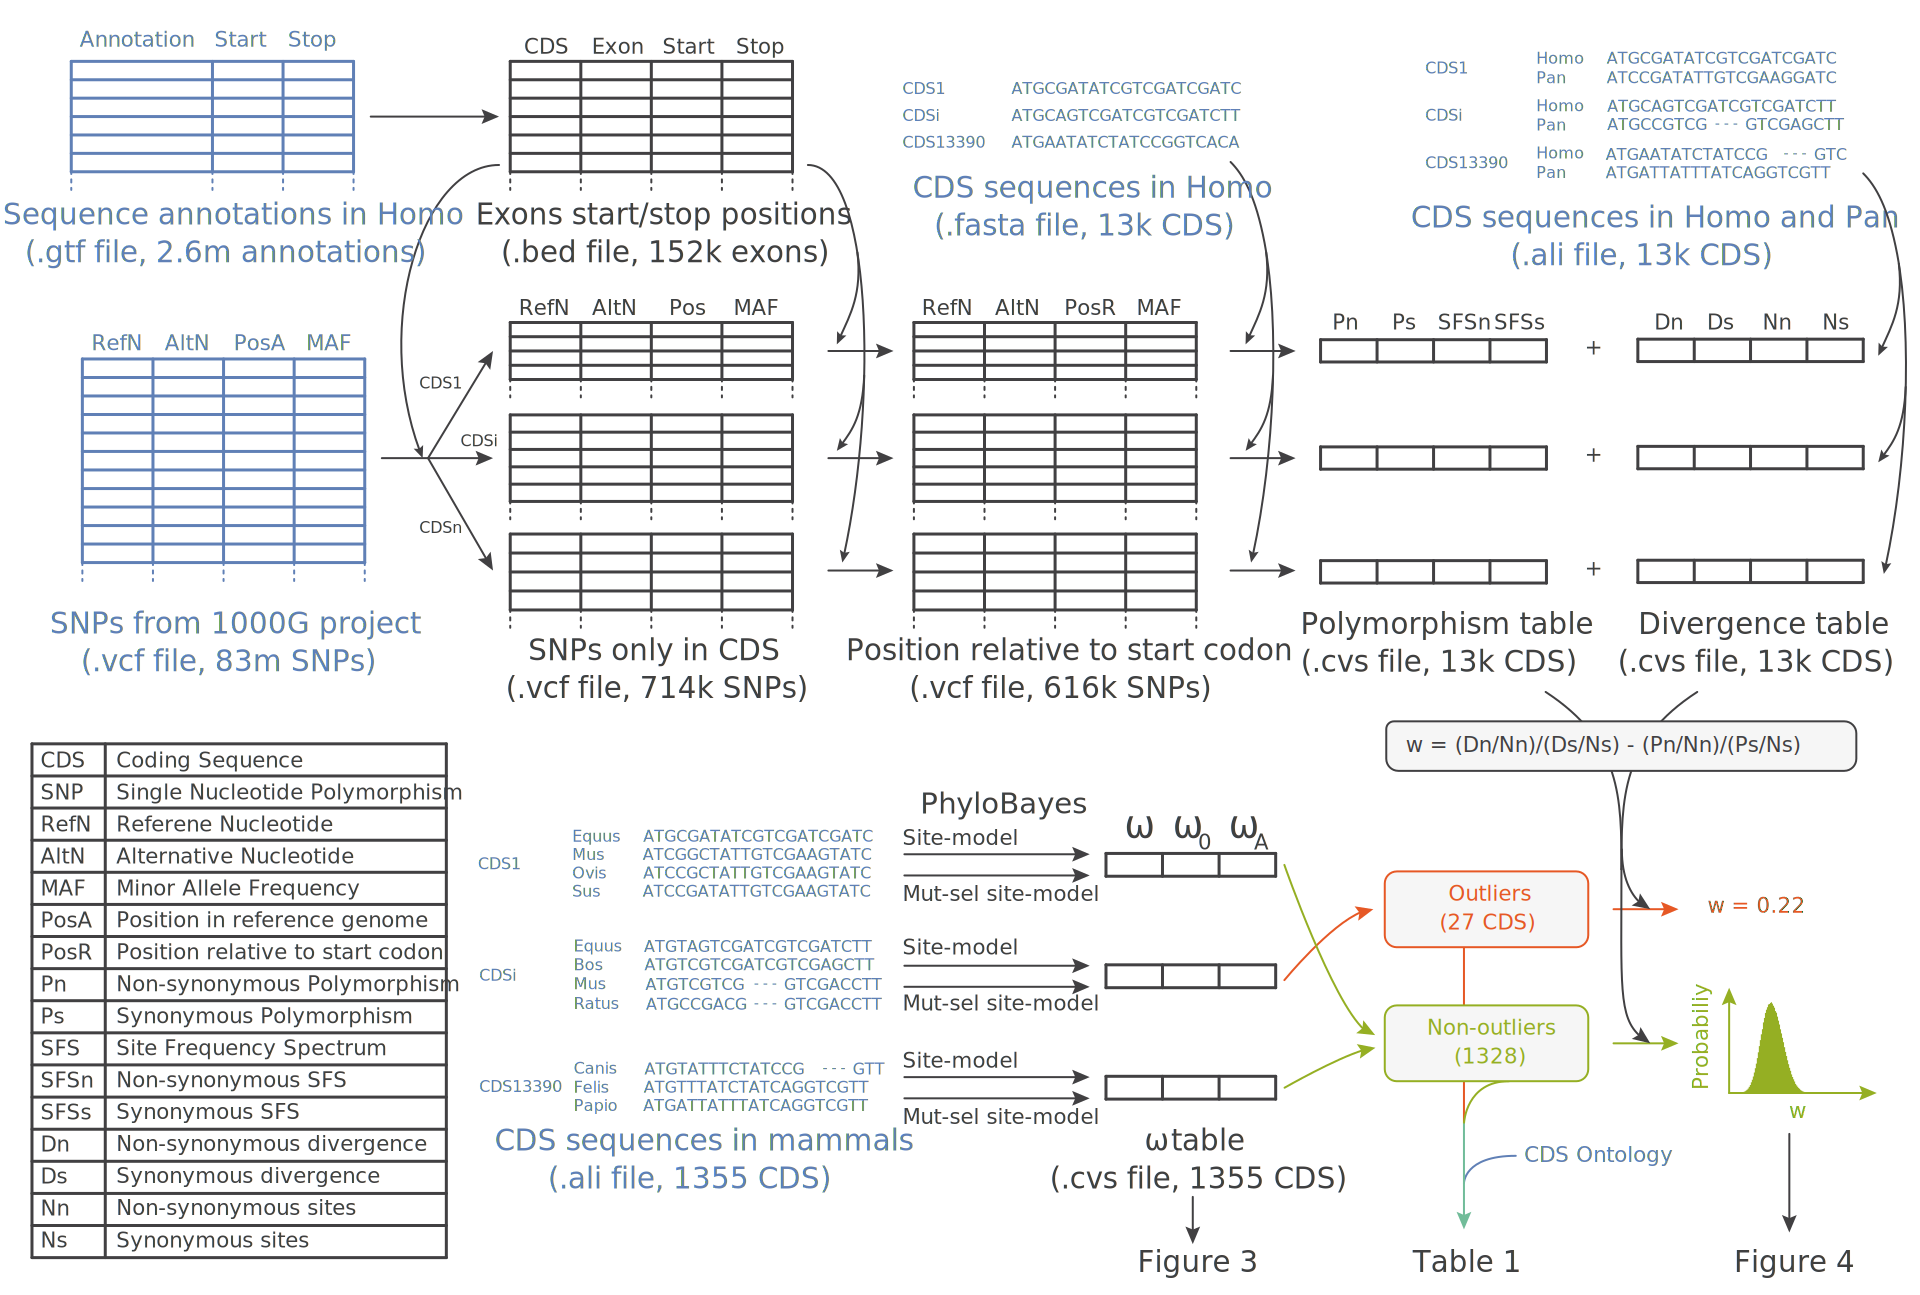
\includegraphics[width=\textwidth]{../Figures/pipeline.pdf}\\
		\caption{ \textbf{The python pipeline for data analysis}. Tables in blue outlines are the input data necessary to run the pipeline. Tables in black outlines are the data produced by the analysis. The upper half of the figure depicts the steps necessary to estimate polymorphism and divergence statistics necessary to run population-based method. The lower half of the figures depicts the steps necessary to run the phylogeny-based method and to obtain figure \ref{fig:omega_pb} and table \ref{fig:ontology}, which can be obtained independently of the population-based analysis. Figure \ref{fig:omega_snp} is obtained by merging the results of the population- and the phylogeny-based analysis. The code available at \href{https://github.com/ThibaultLatrille/AdaptaPop}{https://github.com/ThibaultLatrille/AdaptaPop} allows one to reproduce the figures of this study. \label{fig:pipeline}}
	\end{mdframed}
	\end{figure*}

	\begin{figure*}[hb!]
	\begin{mdframed}
		\centering
		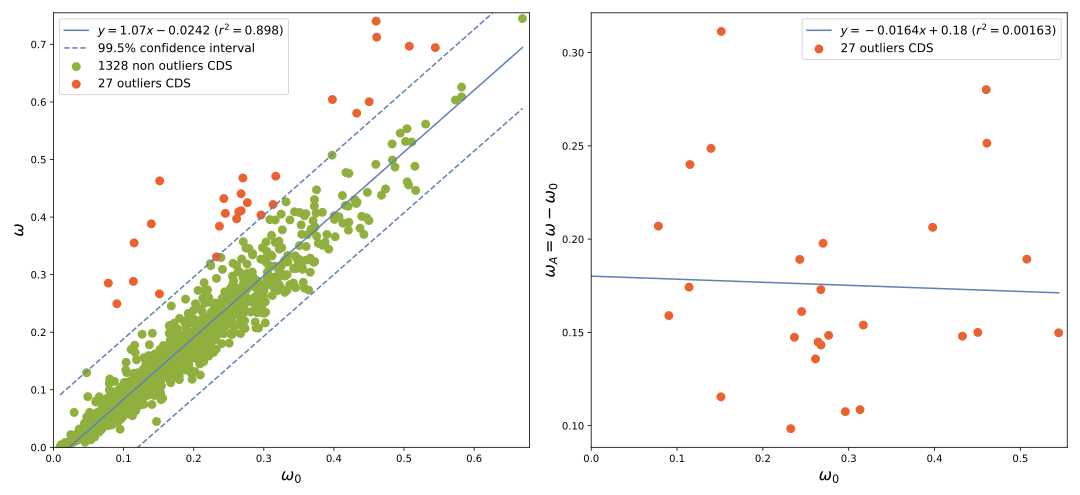
\includegraphics[width=\textwidth]{../Figures/figure_1.pdf}\\
		\caption{ \textbf{Detection of protein-coding sequences ongoing adaptation}. \textbf{Panel A}: scatter plot of $\omega$ (y-axis), such as estimated by the site-model, against $\omega_{0}$ (x-axis), such as estimated by the mutation-selection model for $1,355$ CDS. The linear correlation shows a good empirical fit but outliers (in red) are CDS with significantly high $\omega_A = \omega - \omega_{0}$.  \textbf{Panel B}: for the 27 outliers CDS, scatter plot of $\omega_A$ (y-axis) against $\omega_{0}$ (x-axis). The linear correlation is very poor suggesting that $\omega_A$ effectively extract the adaption regardless of the background of purifying selection ($\omega_0$)  \label{fig:omega_pb}}
	\end{mdframed}
	\end{figure*}


	\subsection*{Theoretical rate of adaption in phylogeny-based method }
	Classical codon models estimate a parameter $\omega=d_N/d_S$, namely the ratio of the non-synonymous over the synonymous substitution rates \cite{Muse1994,Goldman1994}. In the so-called site-models, $\omega$ is allowed to vary across sites, either via a finite mixture \cite{Yang2001}, an infinite mixture \cite{Huelsenbeck2006}, or as random effects from a parametric distribution. In PhyloBayes, the latter option is used: site-specific $\omega^{(i)}$ are independent identically distributed from a gamma distribution \cite{lartillot_phylobayes_2013}. This implementation is used in this study to infer the distribution of $\omega$ across sites on empirical alignments. In a second step, the average over site is calculated, giving estimates of $\omega$ for each protein-coding sequences (see figure \ref{fig:codon_model}, left panel).  \\
	
	In contrast, mutation-selection models assume that the protein-coding sequence (CDS) is at mutation-selection balance under a fixed fitness landscape, which is itself characterized by a fitness vector over the $20$ amino-acid at each site \cite{Yang2008, Halpern1998, Rodrigue2010}. Mathematically, the rate of non-synonymous substitution from codon $a$ to codon $b$ ($q_{a \mapsto b}^{(i)}$) at the $i^{\mathrm{th}}$ site of the sequence is equal to the rate of mutation at site $i$ ($\mu_{a \mapsto b}^{(i)}$) multiplied by the probability of fixation of the mutation ($p_{a \mapsto b}^{(i)}$) \cite{kimura_neutral_1983}. Crucially, the probability of fixation depends on the difference of fitness between the amino-acid encoded by the mutated codon ($f_b^{(i)}$) and the fitness of the amino-acid encoded by the original codon ($f_a^{(i)}$) of site $i$ \cite{wright_evolution_1931, fisher_genetical_1930}. Altogether, the rate of substitution from codon $a$ to $b$ at a given site $i$ is:
	\begin{equation}
		q_{a \mapsto b}^{(i)} = \mu_{a \mapsto b}^{(i)} \dfrac{\mathrm{ln}(f_b^{(i)} / f_a^{(i)})}{1 - f_b^{(i)} / f_a^{(i)}}.
	\end{equation}
	
	Fitting the mutation-selection model on a sequence alignment leads, via equation (1), to an estimation of the mutation rate matrix ($\mu^{(i)}$) as well as the fitness landscape of the protein ($f^{(i)}$) at each site $i$ of the sequence. From these parameters, one can compute $\omega_{0}^{(i)}$, the site-specific predicted rate of non-synonymous over synonymous substitution at the mutation-selection balance: 
	\begin{equation}
	\omega_{0}^{(i)} = \sum_{a \in  \mathcal{C}} \pi_a^{(i)}  \dfrac{\sum_{b \in  \mathcal{N}_a} q_{a \mapsto b}^{(i)}}{\sum_{b \in \mathcal{S}_a} q_{a \mapsto b}^{(i)}},
	\end{equation}
	where $\mathcal{C}$ is the set all the possible codons ($61$ by discarding stop codons), $\pi_a$ is the equilibrium frequency of codon $a$ at site $i$, and $\mathcal{N}_a$ (respectively $\mathcal{S}_a$) is the set of codons that are non-synonymous (respectively synonymous) to $a$  \cite{spielman_relationship_2015, rodrigue_site-heterogeneous_2014}. In a second step, the average over site is calculated, giving estimates of $\omega_0$ for each protein-coding sequences (see figure \ref{fig:codon_model}, right panel). \\
	
	Under the assumption that the protein is under a \textit{nearly-neutral} regime,  the predicted $\omega_0$ (mutation-selection model) and the estimated $\omega$ (site-model) should be the same. But if this assumption is violated, and the protein is under adaptation then $\omega > \omega_0$.
	From these consideration, the method can estimate $\omega_A$, namely the rate of adaptive substitution over neutral substitution as the deviation of $\omega$ from the quasi-neutral model $\omega_0$ (see figure \ref{fig:codon_model}):
	\begin{equation}
		\omega_A = \omega - \omega_0.
	\end{equation}
	
	With this protocol, a two-step procedure is needed and one needs to run independently the site-model and mutation-selection model. An alternative one-step method was proposed originally \cite{Rodrigue2016}, in which a global deviation parameter ($\omega^*$) is directly introduced into the model. Thus equation (1) becomes:
	\begin{equation}
	q_{a \mapsto b}^{(i)} =  \mu_{a \mapsto b}^{(i)} \dfrac{\mathrm{ln}(f_b^{(i)} / f_a^{(i)})}{1 - f_b^{(i)} / f_a^{(i)}} \omega^* .
	\end{equation}
	The null hypothesis correspond to $\omega^*=1$, adaptive evolution to $\omega^*>1$. The rate of adaptive evolution is then:
	\begin{equation}
		\omega_A^* = \omega_0 (\omega^* - 1 ).
	\end{equation}
	In the following, the two approaches will be compared.

	\subsection*{Phylogenetic dataset and experiments}
	Protein-coding sequences (CDS) alignments in $34$ placental mammals were extracted from the \href{http://www.orthomam.univ-montp2.fr}{OrthoMaM} database \cite{ranwez_orthomam:_2007, douzery_orthomam_2014}. A first analysis on $500$ CDS gave inconsistent results since some alignment contained paralogs, frame-shifts and improperly aligned segments. Thus, this study used a dataset cleaned by Fidel Botero-Castro (Institut des Sciences de l'Evolution de Montpellier), where CDS were filtered by HmmCleaner with a threshold of $5$ \cite{di_franco_detecting_2017}. All the CDS with more than $50\%$ of masked nucleotides were discarded, and codon sites masked in more than $40\%$ of the species were also discarded. Finally, each of the $11,256$ CDS of the dataset is at least $500$ bp and includes at least $34$ mammalian species. CDS located on the X, Y and mitochondrial chromosome were also discarded from the analysis, since the number of polymorphism, necessary in population-based method, is expected to be different on these sequences.\\
	
	I ran the Bayesian software \href{https://github.com/bayesiancook/pbmpi2}{PhyloBayes MPI} on randomly chosen $1,355$ CDS from the dataset of Fidel Botero-Castro using the site-model \cite{lartillot_phylobayes_2013} and the mutation-selection model \cite{rodrigue_site-heterogeneous_2014}. Each Monte-Carlo Markov-Chain was ran during $600$ points, with a burn-in of $100$ points. The convergence of the chain during the burn-in was assessed by running two independent chains on preliminary runs, and asserting that parameters of the models of the two chains converged during burn-in. The whole computation took approximately $254,000$ hours of CPU on the LBBE/PRABI cluster. The scripts used for analysis were written in python v3.5.
	
	\subsection*{Theoretical rate of adaption in population-based method}
	In the method proposed by McDonald and Kreitman \cite{McDonald1991}, the ratio of non-synonymous over synonymous polymorphism ($\omega_{0}=p_N/p_S$) only contains non-adaptive polymorphisms. On the other hand, divergence data with regard to a close specie allows one to estimate the ratio of non-synonymous over synonymous substitutions ($\omega=d_N/d_S$) between these species. All the non-synonymous substitutions in the sequence are supposed to be a mixture of both advantageous mutation and non-adaptive substitution. Thus the difference $d_N/d_S - p_N/p_S$ is the rate of adaptive evolution:
	\begin{equation*}
	\omega_A^{MK}=\dfrac{d_N}{d_S} - \dfrac{p_N}{p_S}.
	\end{equation*}\\
		\begin{table*}[hb!]
		\centering
		\begin{adjustbox}{width = 1\textwidth}
			\small\begin{tabular}{|c|c|c|c|c|c|}
				\hline
				Ontology & $n_{\mathrm{Observed}}$ & $n_{\mathrm{Expected}}$ & Odds ratio & $p_{\mathrm{value}}$ & $e_{\mathrm{value}}$\\
				\hline
				plasma membrane & $12$ & $3.48$ & $3.45$ & $0.00232$ & $0.195$\\
				protein heterodimerization activity & $4$ & $0.459$ & $8.71$ & $0.00241$ & $0.202$\\
				regulation of immune response & $2$ & $0.0566$ & $35.3$ & $0.00369$ & $0.31$\\
				T cell differentiation & $2$ & $0.0755$ & $26.5$ & $0.00546$ & $0.459$\\
				immune system process & $6$ & $1.36$ & $4.4$ & $0.00584$ & $0.49$\\
				response to stress & $8$ & $2.24$ & $3.57$ & $0.00608$ & $0.511$\\
				innate immune response & $4$ & $0.659$ & $6.07$ & $0.00765$ & $0.643$\\
				receptor activity & $3$ & $0.348$ & $8.61$ & $0.00845$ & $0.71$\\
				metabolic process & $6$ & $1.51$ & $3.98$ & $0.00899$ & $0.755$\\
				leukocyte migration & $2$ & $0.113$ & $17.6$ & $0.00995$ & $0.836$\\
				\hline
			\end{tabular}
		\end{adjustbox}
		\caption{\textbf{Ontology enrichment in the outliers}. 84 Fisher's exact test were performed with $27$ CDS detected as under adaptation and $1,328$ as under \textit{nearly-neutral} regime. In the table is solely shown the tests with $e_{\mathrm{value}} < 1$. $10$ ontology terms are detected, while one was expected on average, and the estimation of the false discoveries rate is $10\%$. Out of $10$ ontology terms, six terms related to immune processes. \label{fig:ontology}}
	\end{table*}

	However, $\omega_A^{MK}$ can be biased by moderately deleterious mutations \cite{eyre-walker_quantifying_2002} and by the change in population size through time \cite{eyre-walker_changing_2002}. To overcome this biases, the method of Galtier \cite{galtier_adaptive_2016} was used, which relies on the synonymous and non-synonymous site-frequency spectra (SFS) to estimate the distribution of fitness effects of mutations (DFE), modeled as a continuous distribution. The method use a maximum likelihood approach. The GammaExpo model was used, in which the fitness effect of weakly deleterious non-synonymous mutations is distributed according to a negative Gamma. The fitness effect of weakly advantageous mutations is distributed exponentially. This method is an extension of the methods introduced by Eyre-Walker and collaborators \cite{eyre-walker_distribution_2006, eyre-walker_estimating_2009}. This estimation of the DFE than leads to a predicted $d_N/d_S$, under the \textit{nearly-neutral} regime, which can then be subtracted from the $d_N/d_S$ observed between the focal species and its sister group, giving another estimate of the rate of adaptive evolution: $\omega_A^{DFEM}$.
	\subsection*{Polymorphism dataset and experiments}

	Polymorphism in \textit{Homo sapiens} was downloaded from \href{http://www.ensembl.org/index.html}{ensembl.org}. This study relied on the GRCh38 assembly and mutations from the phase 3 of the 1000 genomes projects \cite{consortium_integrated_2012, the_1000_genomes_project_consortium_global_2015}. Mutations not inside CDS were discarded at the beginning of the analysis. Insertions and deletions were not analyzed, and only Single Nucleotide Polymorphism (SNPs) with only one mutant allele were considered. Stop codon mutants were also discarded. Divergence data between \textit{Homo sapiens} and \textit{Pan troglodytes} was extracted from \href{http://www.orthomam.univ-montp2.fr}{OrthoMaM} database \cite{ranwez_orthomam:_2007, douzery_orthomam_2014}. The pipeline (figure \ref{fig:pipeline}) for assembling and analyzing the data is written in python 3.5, the code is under GNU license and available at \href{https://github.com/ThibaultLatrille/AdaptaPop}{https://github.com/ThibaultLatrille/AdaptaPop}. \\
	
	One proposed correction for slightly deleterious polymorphism, in Mc-Donald and Kreitman test, is to drop “rare” polymorphisms, but this method has no clear cut. Dropping singletons provides a simple correction \cite{templeton_contingency_1996}, while other authors have suggested to only include polymorphisms with minor allele frequencies above $10\%$ \cite{smith_adaptive_2002, fay_testing_2002, gojobori_adaptive_2007}. This correction was applied  to compute $\omega_A^{MK}$. In contrast, the model-based method of Galtier to compute $\omega_A^{DFEM}$ allows us to keep all polymorphisms, but since the folded site-frequency spectra (SFS) had $2504$ categories (The 1000G project sequenced $2504$ diploid individuals) the model was then over-parametrized, and the folded SFS were sub-sampled down to $12$ categories using by sampling without replacement (hyper-geometric distribution). The effect of sub-sampling is shown in figure \ref{fig:omega_snp}, panel B.
	

	\section*{Results}
		\begin{figure*}[hb!]
		\begin{mdframed}
			\centering
			\includegraphics[width=\textwidth]{../Figures/figure_3.pdf}\\
			\caption{ \textbf{Empirical distribution of $\omega_A^{MK}$}
				\textbf{Panel A:} $\omega_A^{MK}$ was computed on the concatenate of the $27$ CDS having a high rate of adaptation (outliers, orange solid line), detected in phylogeny-based method. The result was compared to the empirical null distribution of $\omega_A^{MK}$ (green histogram), obtained by randomly sampling a subset of $27$ CDS from the $1,355$ CDS ($100,000$ replicates). The deviation is not significant ($p_{\mathrm{value}}=0.119$).
				\textbf{Panel B:} Sub-sampling the site-frequency-spectrum (SFS) did not affect much the estimation of $\omega_A^{DFEM}$. The dashed line is the $95 \%$ confidence interval around the mean value computed for random sample of $27$ CDS.
				\textbf{Panel C:} Synonymous versus non-synonymous folded SFS,  sub-sampled down to $12$ categories. On top the SFS in the $27$ outliers. On bottom the SFS of all CDS.
				\textbf{Panel D:}. $\omega_A^{DFEM}$ was computed on the concatenate of the $27$ CDS having a high rate of adaptation (outliers, orange solid line), detected in phylogeny-based method. The result was compared to the null empirical distribution of $\omega_A^{DFEM}$ (green histogram), obtained by randomly sampling a subset of $27$ CDS from the $1,355$ CDS ($100,000$ replicates). \label{fig:omega_snp}}
		\end{mdframed}
	\end{figure*}
	\subsection*{Detecting protein-coding sequences under adaptation}
	Using a randomly chosen set of CDS, I first assessed the performance of the phylogeny-based method. Such as originally proposed \cite{Rodrigue2016}, the mutation-selection model approach relies on a one-step method to jointly estimate the nearly neutral null model and the deviation from it (through a deviation parameter $\omega^*$ from which the method can estimate $\omega_A^*$, see methods). However the application of this one-step approach on the set of $1,355$ CDS led to results that were difficult to interpret. In particular, a reasonable expectation is that $\omega_A$ should be either close to zero (\textit{nearly-neutral} regime) or positive (adaptation). However, is should never be strongly negative. Yet this was observed for several CDS, suggesting a statistical artifact of the method. More specifically, $\omega^*$ captured part of the purifying process which is normally supposed to be modeled at the level of the amino-acid fitness profiles, for these proteins $\omega^*$ was very close to zero, thus resulting in $\omega_A^*<0$.  \\
	
	Accordingly, I derived a two-step approach (see methods), which was applied to the set of CDS. In contrast to the one-step method, the results obtained here are more sensible. The value of $\omega$ estimated by the site-model and of $\omega_{0}$ estimated by the mutation-selection model show a good linear correlation ($r^2=0.898$) indicating that, for most protein, the mutation-selection site-model effectively predicts the rate of non-synonymous substitutions over the rate synonymous substitutions. The \textit{nearly-neutral} assumption is thus not rejected for most proteins (see figure \ref{fig:omega_pb}, left panel).
	On the other hand, a few proteins appear to have an actual $\omega$ substantially higher that of the $\omega_0$ predicted by the mutation-selection model (point above the regression line). Assuming that most proteins are essentially under a \textit{nearly-neutral} regime, the analysis takes the distribution of residual errors around the regression line, and compute the $99.5\%$ confidence interval around the predicted value $\omega$ (dashed blue lines).  The method detected $27$ CDS having a value of $\omega$ above the upper bound of the confidence interval, meaning that the value of their $\omega$ is too high compared to $\omega_{0}$. For this threshold of $99.5\%$, $6.78$ CDS are expected to outside the confidence interval and therefore the estimated false discovery rate is around $25 \%$. For the outliers, the nearly neutral-model assumption appears to be rejected, and those proteins are putatively under ongoing adaptation. Of note, the method detected no CDS with $\omega$ below the lower bound of the confidence interval. \\
	
	In the set of outliers, I computed  $\omega_A = \omega - \omega_0$, and asserted that $\omega_A$ correlates poorly with $ \omega_0$ ($r^2=0.002$), suggesting that $\omega_A$ effectively extract the adaption regardless of the background of purifying selection (see figure \ref{fig:omega_pb}). \\
	
	\subsection*{Ontology enrichment tests}
	Next, I investigated whether the outliers CDS showed enrichment in ontology terms. Thus, on the set of outliers, I performed Fisher's exact test to estimates ontology enrichment by contrasting with the set of all CDS (see figure \ref{fig:ontology}). $10$ ontologies were observed with an $e_{\mathrm{value}} <1$, while in expectation $1$ ontology term should have observed if ontology terms were assigned randomly. The estimated false discovery rate is therefore around $10 \%$. Among these $10$ ontology terms, $60 \%$ were related to immune processes. An enrichment in CDS involved in immune processes was also found in large scale analysis based on classical site codon-models ($16,529$ CDS, Kosiol \textit{et al} \cite{kosiol_patterns_2008}). \\
	
	Altogether, the mutation-selection method effectively detects adaptation regardless of the background of purifying selection, and returns reasonable candidates for adaptive evolution. 	

	\subsection*{Congruence between phylogeny- and population-based methods}
	Finally, I investigated whether the phylogeny-based and the population-based methods give congruent results in terms of detection of adaptive evolution. 
	To do so, $\omega_A^{MK}$ was computed on the concatenate of the $27$ candidates CDS inferred, by the phylogeny-based method, to have a high rate of adaptation. The result was compared to the empirical distribution of $\omega_A^{MK}$ over random sets of $27$ CDS (see figure \ref{fig:omega_snp}, panel A).
	The average rate of adaptation over the $27$ candidates, such as estimated by Mc-Donald and Kreitman (see methods), is higher than the average rate of adaptation over random samples. However, the deviation is not significant ($p_{\mathrm{value}}=0.119$).\\
	
	Similarly, using the site-frequency spectra of SNPs, $\omega_A^{DFEM}$ was computed in the same set of candidates by concatenating the $27$ site-frequency-spectrum (see figure \ref{fig:omega_snp}, panel C). And compared it to the empirical null distribution of $\omega_A^{DFEM}$ over random sets of $27$ CDS (see figure \ref{fig:omega_snp}, panel D).
	The average rate of adaptation over the $27$ candidates, such as estimated using the GammaExpo model (see methods), is higher than the average rate of adaptation over random samples. In this case, the deviation is marginally significant ($p_{\mathrm{value}}=0.036$), 
	meaning that modeling change in population size and the distribution of fitness effects of mutations leads to more congruence between phylogeny- and population-based methods, suggesting that the two methods are at least partially congruent in their detection of adaptation.
	
	\section*{Discussion}


	This study is the first medium-scale application of the phylogenetic mutation-selection method for detecting adaptation. The approach required some changes compared to the original method. More specifically, a two-step procedure was derived and deemed more reliable than the one-step \cite{lartillot_phylobayes_2013}. This approach seems to give sensible results. Its application on mammalian CDS suggests that most proteins are under \textit{nearly-neutral} regime and a few candidate proteins are under strong adaptation. The protein under adaptation also showed significant increase in ontology terms related to immune processes. In practice, there could be some background adaption in proteins categorized here as being in a \textit{nearly-neutral} regime, which might not have been detected due to lack of power of the statistical test. Further work is also needed to compare with classical codon models. Here, $27$ CDS were detected out of $1,355$. In Kosiol \textit{et al} \cite{kosiol_patterns_2008}, $400$ CDS were detected out of $16,529$ using codon site-model, suggesting that the mutation-selection model has somewhat a lower, although comparable, sensitivity compared to site-model. Ultimately, I should first scale-up the analysis to the whole dataset of $11,256$ CDS, instead of the $1,355$ CDS used because of time and computation constrains. Indeed, phylogeny-based method is computationally intensive, and requires a well resolved species tree, hence the limitation to mammals in this study. Moreover it crucially depends on the quality of the alignments, as was observed in preliminary study, and paralogs identified as orthologs or alignment problems can easily falsify the results.\\
	
	A second objective of this work was to confront phylogeny-based and population-based methods. One main novelty of mutation-selection model, compared to classical codon models, is to provide an estimate of $\omega_A$, thus directly comparable with population-based methods. Ideally, one would like to make a quantitative comparison of $\omega_A$ and $\omega_A^{MK}$, across sequence or groups of sequences. However, the method lacked of power for two reasons. Firstly, the method did not detected enough CDS under adaptation ($27$ CDS with $\omega_A > 0$). Secondly the population-based estimation was very noisy, also requires concatenating many sequences. Nevertheless, these preliminary results are encouraging. Practically, it is possible to apply this pipeline to other species than \textit{Homo sapiens}, where polymorphic diversity is greater such as \textit{Mus} (using the same mammalian phylogeny) or \textit{Drosophila} (with another phylogeny). \\
	
	The set of CDS detected to be under adaptation in phylogeny-based methods showed a marginally significant increase in the rate of adaption, such as inferred by population-based method. This relatively weak correlation might just reflect the limited number of CDS analyzed and the limited statistical power of the population-based method mentioned above. However, it is also possible that the two methods are inherently testing for different patterns of adaptation, meaning that recent episode of adaptation in the \textit{Hominini} lineages do not reflect the long-term patterns of adaptation. Especially since the purifying process is stronger on longer timescale, the frontier between neutral and mildly deleterious mutation is blurred on short timescale \cite{ho_time_2005}. \\
	
	Altogether, this preliminary study suggest that the integration between population and phylogeny-based methods raises theoretical and practical issues. I suggest that further investigating these methodological integration will provide biological understanding of the evolutionary constrain of protein-coding sequences. \\
	
	\section*{Author contributions and acknowledgments}
	I thank Nicolas Lartillot for his help, support and advises all along the internship and concerning this report, as well as for insightful discussions. I thank the team for the great atmosphere at the lab, and Fidel Botero-Castro for providing cleaned mammalian alignment data. The personal equipment was provided by ANR Dasire. This work was performed using the computing  facilities of the CC LBBE/PRABI. I wrote all the python code of the pipeline (figure \ref{fig:pipeline}), and I designed the statistical tests and analyzed the data. The repository for the pipeline and this report is available at \href{https://github.com/ThibaultLatrille/AdaptaPop}{https://github.com/ThibaultLatrille/AdaptaPop}.

	\bibliographystyle{unsrt}
	\bibliography{codon_models,adaptapop}
	
	\end{multicols}
\end{document}
